\chapter{Les archives au Luxembourg~: législation récente et traitements urgents qui poussent vers l’exploration de moyens d’automatisation}

\subsection{Un cadre légal récent}


La réglementation sur la conservation des archives est récente au
Luxembourg. Le sujet a longtemps été ignoré. Ce manque d'attention est lié à
l'histoire du pays. Jusqu\textquotesingle à
l'abolition du secret bancaire par une loi votée le 5 novembre 2014, le
secret y prévalait sur la transparence. Cette culture persiste. Il faut
encore aujourd'hui davantage justifier la conservation des documents que
leur destruction. Cette situation a influencé la gestion des archives
et nous l'avons perçu pendant notre stage. Par exemple, les archivistes
doivent demander un accès aux données sensibles stockées sur les
serveurs métier et la demande n'est pas toujours acceptée.
Archiver des documents contenant des données sensibles est un défi
malgré les exceptions prévues par l\textquotesingle article 89 du RGPD,
qui octroie des dérogations pour le traitement \enquote{à des fins
archivistiques dans l\textquotesingle intérêt public, à des fins de
recherche scientifique ou historique ou à des fins
statistiques\footcite{EuropeanParliament2016a}}. Pour illustrer la difficulté de l'archivage à la Chambre, 
nous pouvons mentionner le cas des archives de Fernand Etgen,
président de la Chambre de 2018 à 2023, qui n'ont pas été récupérées. 

Le consensus tient par ailleurs une place importante dans
le processus politique luxembourgeois. Les lois doivent être discutées et approuvées
collectivement, et non imposées. Le processus législatif se
déroule comme suit~: les textes de loi sont étudiés par une ou plusieurs
Commissions parlementaires, qui peuvent les amender, et sont ensuite
généralement transmis pour avis à des Chambres professionnelles et au
Conseil d'État. Le texte est plus tard débattu en séance publique. Il peut
être amendé à ce moment-là aussi si nécessaire, puis il est voté en
séance plénière\footcite{noauthor_chambre_2024}. Ce besoin de consensus a pu contribuer à
ralentir le processus de législation sur les archives.
\newline

En ce qui concerne l'histoire des archives au Luxembourg, la
constitution d'un véritable fonds d'archives publiques
remonte à la loi du 5 brumaire de l'an V (26 octobre 1796), quand la
région était sous l'administration française. Ce
n\textquotesingle est qu\textquotesingle avec la loi du 5 décembre 1958
que les « Archives de l'État » obtiennent une forme de base
légale\footcite{loi_1958}. En 1988, rebaptisées « Archives
nationales », elles reçoivent le statut d\textquotesingle« institut
culturel »\footcite{loi_1988}. Une loi adoptée le 25 juin 2004 sur
la réorganisation de ces instituts culturels détaille les missions des
Archives nationales~: elles ont non seulement un rôle de collecte et de
conservation, mais aussi de sensibilisation, de conseil et d'encadrement
des détenteurs d'archives, publiques ou privées. Elles ont également un
rôle scientifique~: elles doivent organiser des expositions ou des
colloques. Elles doivent accepter des archives publiques ou «~privées
d'intérêt historique, scientifique, économique, sociétal ou
culturel\footcite{loi_2004}~». Elles doivent enfin
\enquote{contribuer au développement de l'archivistique au niveau national et
au niveau international\footcite{loi_2004}}.

 La plus grande
avancée législative arrive avec la loi du 17 août 2018, qui établit pour
la première fois un réel cadre légal pour les archives publiques au
Luxembourg. Cette loi fixe des règles concernant \enquote{la gestion, la
conservation, la communication, le versement et la destruction des
archives publiques\footcite{loi_2018}}. Les
archives publiques doivent être gérées de manière à garantir leur
pérennité, accessibilité et
lisibilité tout au long de leur cycle de vie. La loi attribue aux
Archives nationales du Luxembourg (ANLux) une mission d'encadrement des
producteurs d'archives publiques. L'article 4
distingue deux types de régimes pour les producteurs~: le régime général
et le régime dérogatoire.
Les établissements soumis au régime dérogatoire gèrent et
conservent eux-même leurs archives, alors que les établissements soumis
au régime général doivent proposer le versement aux ANLux. Ces régimes
ont été créés en vertu de la séparation des pouvoirs. Le régime général
concerne les administrations et services de l'État. Les administrations
qui représentent les autres pouvoirs sont soumises au régime
dérogatoire. C'est donc le cas de la Chambre des Députés, représentante
du pouvoir législatif. Cette législation est révélatrice d'une prise de
conscience de l'importance des archives, mais surtout du pouvoir de
l'information, qui fait aussi écho au passé de paradis fiscal du pays.
Cette conscience devrait favoriser un meilleur traitement des archives,
toutefois, une certaine peur de la diffusion d'informations sensibles
subsiste. La transparence est promue pour lutter contre cette
image du secret. Elle est mentionnée dans l'article premier de la loi.
\newline

L'État a à cœur de développer un esprit de transparence, qui passerait
par une bonne conservation et communication des archives. Des efforts
restent malgré tout à fournir pour atteindre cet objectif. En ce qui
concerne la communication, la loi de 2018 fixe des délais de
communicabilité pour les archives définitives. Les archives sont
consultables par les citoyens passés ces délais. Des dérogations peuvent
également être demandées pour avoir un accès aux documents avant qu'ils
soient échus. Les délais de communicabilité sont exposés dans l'article
16. Ils sont les suivants~:

\begin{longtable}{|p{0.45\textwidth}|p{0.5\textwidth}|}
    \tableheader{Type de donnée}{Délai de communicabilité}
	
	Données à caractère personnel & 25 ans après le décès de la personne concernée ou 75 ans à compter de la date du document le plus récent inclus dans le dossier \\
	\hline
	Actes d'état civil & 100 ans à partir de la date de l'acte \\
	\hline
	Actes notariés & 75 ans à partir de la date de l'acte \\
	\hline
	Atteinte aux relations extérieures, à la sécurité du Grand-Duché ou à l'ordre public & 50 ans à compter de la date du document le plus récent inclus dans le dossier \\
	\hline
	Affaires portées devant les instances juridictionnelles, extrajudiciaires ou disciplinaires & 50 ans à compter de la date du document le plus récent inclus dans le dossier \\
	\hline
	Prévention, recherche de faits punissables & 50 ans à compter de la date du document le plus récent inclus dans le dossier \\
	\hline
	Données commerciales et industrielles & 50 ans à compter de la date du document le plus récent inclus dans le dossier \\
	\hline
	Secret fiscal & 100 ans à compter de la date du document le plus récent inclus dans le dossier \\
	\hline
\end{longtable}



L'inventaire des Archives nationales, dont notre stage avait pour but
d'automatiser le remplissage, est la conséquence de l'établissement de
ces délais. Chaque colonne correspond à un type de document listé dans la loi, qui ne donne que peu de précisions sur ces différentes typologies. Cela a parfois complexifié notre travail. Nous avons
dû réaliser un effort plus approfondi de définition des 
typologies mais leur subjectivité est demeurée problématique. Elle est abordée plus en détail dans la partie 3.1.2. de la note méthodologique en annexe. Un travail plus approfondi de définition
est à réaliser et a été commencé par les Archives nationales. Une
nouvelle loi sur l'archivage est également en préparation, elle pourrait
être l'occasion d'apporter davantage de précisions. Une consultation
publique a été organisée en avril 2024. Le manque de
précision des attentes réglementaires en matière d'archivistique peut
être un obstacle en cas d'automatisation. Les résultats des
tentatives d'automatisation seront réellement précis lorsque les
définitions seront précises. Toutefois, la loi de 2018 fixe un
cadre qu'il était nécessaire de mettre en place afin d'harmoniser les
pratiques archivistiques publiques, mais surtout d'assurer la
conservation et la communicabilité des archives, composante essentielle
dans une démocratie qui met en avant la transparence. 

Beaucoup de
traitements sont à réaliser pour atteindre ces objectifs. Nous avons
déjà abordé le remplissage d'inventaires, permettant d'obtenir une forme
de description archivistique et de gérer les délais de communicabilité.
L'article 6 de la loi de 2018 impose l'établissement de tableaux de tri,
dont la rédaction est à la charge des établissements lorsqu'ils sont
soumis au régime dérogatoire. D'autres traitements sont également
prioritaires dans les administrations. Il faut classer les archives. A
la Chambre des Députés, les projets prioritaires de la Cellule archives sont
actuellement le tableau de tri et le plan de classement. Une première
version du tableau sera bientôt publiée. Une ébauche de plan de
classement a été réalisée pour un service, le Service des relations
européennes, internationales et du protocole (SREIP). La Cellule
archives de la Chambre a encore du travail à faire pour assurer une
bonne conservation et communication de ses archives. C'est pourquoi
les projets d'automatisation sont bienvenus. C'est également le cas pour
d'autres services d'archives publiques. Au moment de la rédaction de ce
mémoire, le seul régime dérogatoire dont le tableau de tri est
disponible sur le site internet des Archives nationales est celui de la
Commission consultative des Droits de
l\textquotesingle Homme.\footnote{ANLux, «~Tableaux de tri~», URL~:
	\url{https://anlux.public.lu/fr/gerer-ses-archives/tableaux-de-tri.html},
	Consulté le 07/08/2024.}. Les services d'archives doivent également se rendre visibles et faciliter la recherche dans leurs fonds. Dans cette optique, des portails numériques d'archives émergent. Les archives communales de Differdange ont par exemple lancé le leur en 2022, permettant d'accèder à des registres numérisés et à des galeries thématiques d'images\footnote{VLA,
	 «~Nouveau portail des archives communales de Differdange !~»,	URL~: \url{https://www.archives.lu/media/Accueil/Nouveau\%20site\%20internet_Archives\%20communales\%20de\%20Differdange_com.pdf},
	Consulté en 24/08/2024.}.
\newline

La loi du 17 août 2018 mentionne par ailleurs la sous-traitance privée. Les
producteurs ou détenteurs d\textquotesingle archives publiques peuvent
en effet externaliser leur conservation à un sous-traitant privé. Ils
doivent informer les Archives nationales de l\textquotesingle identité
et de la durée du contrat du sous-traitant. Les régimes dérogatoires
doivent conserver eux-mêmes leurs archives destinées à être conservées
définitivement\footcite{loi_2018}. Le traitement des
archives par des entreprises privées spécialisées est récurrent au
Luxembourg. Ce recours au privé permet de combler le manque de
personnel et de formation de ce dernier. 

À la Chambre des Députés, la première personne
chargée de la gestion des archives avec une formation archivistique est arrivée en
2008. Avant cela, une personne sans formation avait travaillé sur les
dossiers parlementaires, le reste des documents n'avait pas été traité.
Une deuxième archiviste a été recrutée en 2023. La Cellule archives est
vouée à s'agrandir prochainement. 

Il n'y a pas de formation
archivistique au Luxembourg. La plupart des archivistes viennent de
France, de Belgique ou d'Allemagne. Un concours existe pour les
conservateurs des archives. Il est la plupart du temps destiné et
obtenu par des historiens. Beaucoup d'archivistes luxembourgeois sont
formés en France à l'INP (Institut national du patrimoine) via le Stage
technique international d\textquotesingle archives, dont le rythme est
de deux modules de deux heures par semaine pendant un mois à distance et
d'environ quinze jours de cours\footnote{INP, «~Stage technique
	international d\textquotesingle archives (STIA)~»,URL~:
	\url{https://www.inp.fr/stage-technique-international-darchives-stia},
	Consulté le 07/08/2024}. L'archivistique luxembourgeoise n'est pas
encore dans une période de maturité. Elle se nourrit de différentes
pratiques. Le dialogue entre les pratiques des différents pays et le
fait qu'il existe un recul sur ces dernières est un facteur intéressant.
Le Grand-Duché a une opportunité de capitaliser sur l'expérience de
différentes régions pour construire ses propres pratiques. 
\newline

Les défis de gestion des archives au Luxembourg sont donc nombreux
pour un domaine longtemps négligé. Ils mettent en lumière
l\textquotesingle importance de l\textquotesingle exploration de moyens
d\textquotesingle automatisation qui permettraient d'y répondre. La récurrence de la sous-traitance rend ces perspectives encore plus attrayantes
pour les producteurs d'archives publiques, leur permettant de ne pas
dépendre du privé, d'être ainsi davantage maîtres de leur données et
de réaliser des économies.



\subsection{Les enjeux des archives numériques~: un territoire peu exploré et de nouvelles données à appréhender}

Les archives sont définies dans la loi du 17 août 2018 comme
«~l\textquotesingle ensemble des documents, y compris les données, quels
que soient leur date, leur lieu de conservation, leur forme matérielle
et leur support, produits ou reçus par toute personne physique ou morale
et par tout service ou organisme public ou privé dans
l\textquotesingle exercice de leur activité\footcite{loi_2018}~». Les documents et données numériques sont donc inclus dans la notion d'archive.
Une loi a été consacrée aux documents électroniques. Il s'agit de la loi
du 25 juillet 2015 relative à l'archivage électronique. Cette loi définit les règles
pour garantir l\textquotesingle intégrité, la confidentialité et la
valeur probante des copies numériques, équivalentes à celles des
originaux\footcite{loi_2015}. Elle encadre l'activité des
Prestataires de Services de Dématérialisation et de Conservation (PSDC),
imposant leur certification et leur inscription auprès de l'ILNAS
(Institut Luxembourgeois de la Normalisation, de l'Accréditation, de la
Sécurité et qualité des produits et services)\footcite{loi_2015}. Cette loi est donc centrée sur la question de la valeur
juridique des documents électroniques et non sur leur traitement et elle n'est pas orientée vers le secteur public,
seulement vers le privé. L'idée
du pouvoir de l'information prévaut de nouveau, les valeurs scientifiques ou
patrimoniales des archives sont ici ignorées. Elles sont en effet
d'autant plus complexes à faire reconnaître lorsque l'on traite de
documents numériques. Les archives
électroniques ne sont ici réglementées que lorsque et parce qu'elles ont un
équivalent papier. Les archives nativement numériques restent ainsi à
appréhender chez les producteurs d'archives publiques luxembourgeois.
Les premiers systèmes d'archivage électronique (SAE) émergent, dont un
SAE mis à disposition par le CTIE (Centre des Technologies de l'Information de l'Etat) 
pour les administrations du secteur public. L'inventaire qui a fait l'objet
de notre stage est quant à lui lié au système d'information archivistique (SIA) des ANLux. Il permet d'automatiser la
communicabilité des archives qui y sont rentrées. À la Chambre des Députés, il n'y a
pas encore de système d'archivage électronique mais il est en projet. Comme
évoqué précédemment, les archivistes travaillent aussi sur un plan de
classement des documents numériques.

Le chantier du numérique est mené en parallèle d'autres chantiers dans
les services d'archives publiques. Il faut d'abord sécuriser la collecte
et la conservation des documents papier. Les documents anciens, et par
conséquent souvent fragiles, ont été priorisés. Il est plus aisé de
lancer des projets de traitement de ce type de documents parce que les
personnes qui ne viennent pas du milieu archivistique y voient davantage
d'intérêt historique. Les documents numériques ont toutefois autant de
valeur historique. On pourrait de plus argumenter que le numérique aussi
revêt une certaine fragilité. Malgré les possibilités de traçage des
opérations, il est facile de supprimer, de reclasser et de modifier des
documents stockés sur des serveurs sans que qui que ce soit ne s'en rende
compte. Le passage d'un document d'un système informatique à un autre
peut aussi entraîner des pertes de données. Il existe des moyens de
vérifier l'intégrité des documents, par exemple en calculant
un \emph{hash}, code en principe unique généré à partir du contenu du fichier via un algorithme, qui
permettra de détecter toute modification par comparaison. Certains formats de fichiers
peuvent également être difficiles à ouvrir parce que ce sont des formats
obsolètes ou propriétaires. Les formats sont divers et les manières de les
traiter peuvent varier~: une boîte mail ne sera pas traitée de la même
manière qu'une arborescence de fichiers bureautiques ou qu'une base de
données. Certains supports sont par ailleurs fragiles. C'est par exemple
le cas du CD-ROM qui se dégrade parfois en une dizaine d'années. Par
ailleurs, un document numérique est soit lisible soit
illisible\footcite{noauthor_scarcity_2003}. Il n'y a pas
d'entre deux, pas de dégradation lente qui pourrait sonner un signal
d'alarme, contrairement au papier. Les liens entre les documents sont
eux aussi fragiles. Un exemple concret est celui du déplacement d'un tableur
d'un dossier numérique à un autre~: si ce tableur contient des formules
faisant référence à un autre document du même dossier, le lien peut être
rompu. Les formules et macros posent aussi des soucis. Il faut donc prendre un certain nombre de précautions
face aux documents électroniques. De plus, le numérique évolue vite. Une
veille constante est à réaliser sur les technologies utilisées dans les
administrations et sur les technologies de traitement des archives. De
nouvelles données sont constamment ajoutées sur les serveurs et
dans le \emph{cloud} des administrations. Une autre question se pose face à
cette mutabilité~: quand archiver définitivement~? Cette question
concerne par dessus tout les archives du web, dont les sites sont
constamment actualisés\footcite{wieringa_fragility_2017}. La solution
trouvée est la collecte régulière, ou bien le traçage des modifications.
La Chambre doit encore décider si elle archive son propre site web malgré les 
opérations de capture effectuées par la Bibliothèque nationale du Luxembourg (BNL). 
Ce sera une possibilité à éventuellement
explorer. Les documents numériques revêtent donc une certaine fragilité
et leur traitement doit donner lieu à des réflexions spécifiques.

Les traitements ne sont pas les mêmes que pour des supports matériels.
De nouvelles méthodologies sont à mettre en place et de nouvelles
compétences sont à développer au sein des équipes\footcite{noauthor_prise_nodate}. De nouvelles normes
seront à adopter d'après certains archivistes\footcite{rajotte_reflexion_2010}. Les
Archives nationales du Luxembourg tentent de guider les producteurs
d'archives publiques sur l'archivage numérique, notamment sur les étapes
de traitement de vracs. Les difficultés de traitement des vracs numériques ont été résumés dans un guide publié par l'AAF (Association des archivistes français)\footcite{bechard_archives_2020}. 
En voici un résumé non exhaustif :
\begin{itemize}
	\item Copies et versions multiples des documents
	\item Structuration anarchique et gros volumes à traiter
	\item Variété des formats de fichiers
	\item Existence de fichiers corrompus
	\item Valeurs dynamiques et accès restreints aux documents
	\item Présence de données sensibles
	\item Absence de traçabilité des opérations sur les données
\end{itemize}
Nous avons eu l'occasion de discuter avec plusieurs membres du service \enquote{Collecte, conseil et encadrement} des ANLux des traitements à fournir face à ces problématiques. Nous les avons regroupés en une illustration ci-dessous. Les ANLux travaillent sur des moyens d'automatisation de ces différentes
étapes. Plus d'une trentaine de scripts \emph{shell} ont été développés et
sont diffusés auprès des producteurs d'archives publiques. Ils ont en
partie été réalisés à l'aide de l'intelligence artificielle\footcite{IA_porte}. Les
Grands modèles de langage sont en effet performants pour la génération
de programmes informatiques. Les scripts interviennent pour classer, trier et vérifier l'intégrité des archives\footcite{IA_porte}. La figure 2 ci-dessous, extraite de la note
méthodologique, liste divers moyens d'automatisation de traitements de vracs numériques,
 incluant des scripts créés par les ANLux.

\begin{figure}[h!]
	\centerline{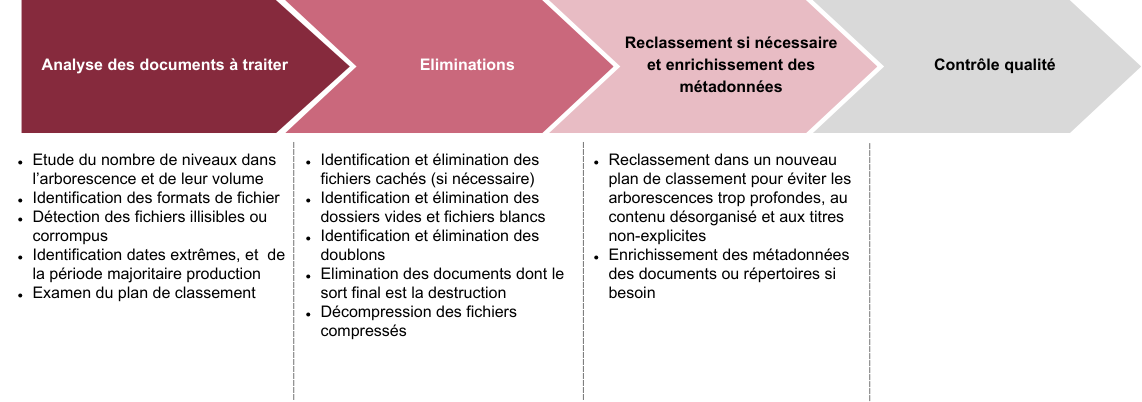
\includegraphics[width=\textwidth]{./media/image1.png}}
	\caption{Étapes de traitement des vracs numériques identifiées pendant le stage}
\end{figure}

\begin{figure}[h!]
	\centerline{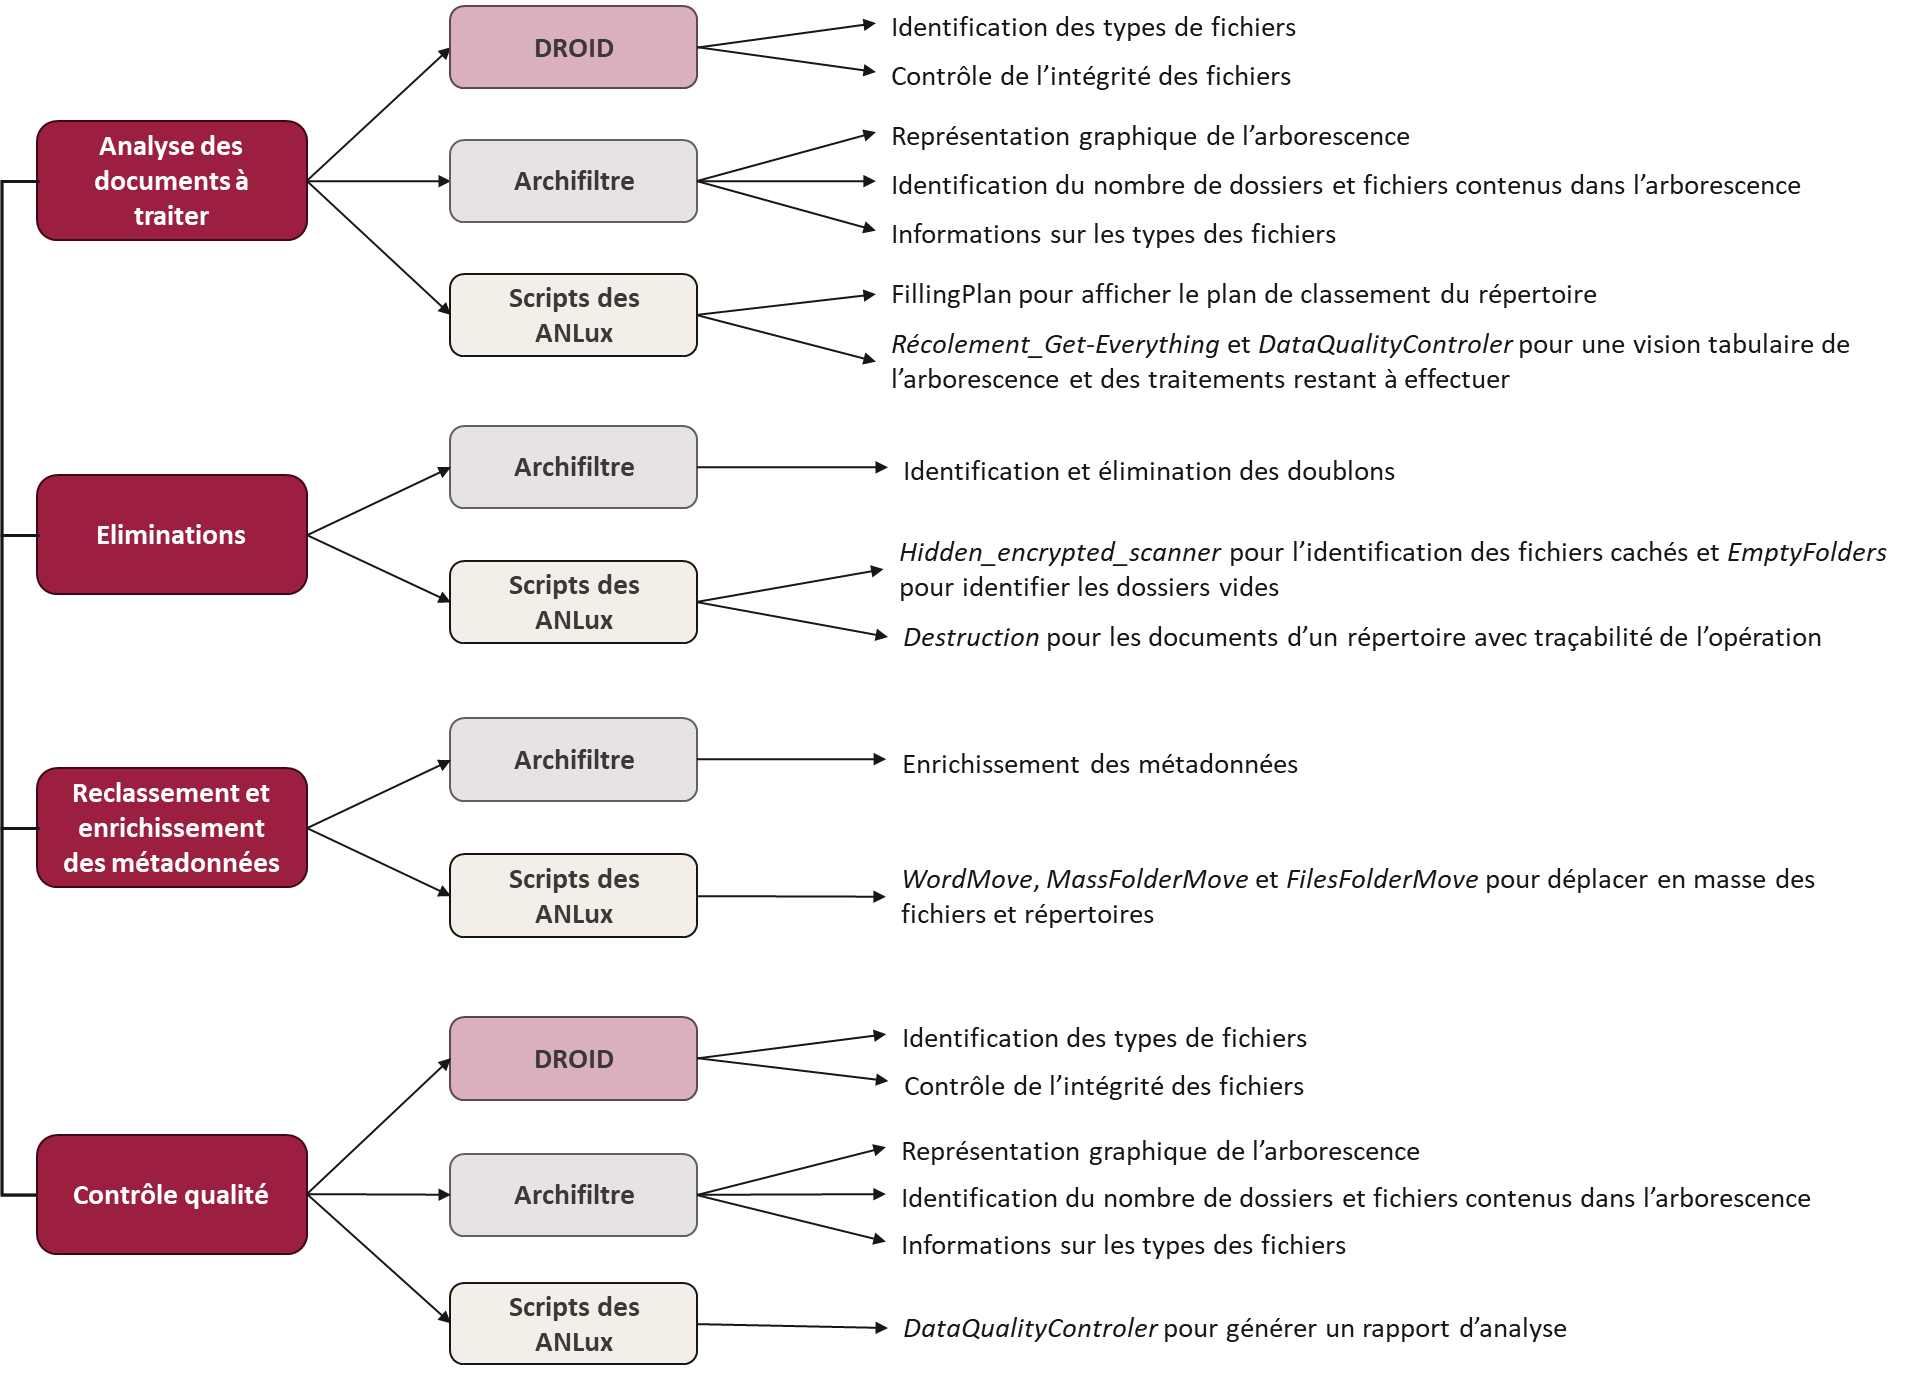
\includegraphics[width=\textwidth]{./media/image2.png}}
	\caption[note]{Moyens d'automatisation par étape de traitement de vracs numériques \footnotemark }
\end{figure}


La réalisation de l'inventaire vient après ces traitements. Une fois les
archives prêtes à être conservées, elles doivent être décrites et les
données sensibles doivent être repérées. L'ensemble de ce travail
nécessite du temps et des moyens, mais ils sont de moins en moins considérables grâce aux outils d'automatisation. 
L'article présentant le travail des ANLux en termes d'automatisation évoque qu'
 \enquote{en 2022, un vrac de 350 Go a nécessité près de 60 jours alors qu'en 2023, un vrac de 1,2 To n'en prenait que 20.\footcite{IA_porte}} 
En ce qui concerne l'inventaire, les
archivistes de la Chambre avaient calculé qu'il faudrait sept ans à
temps plein pour rédiger les inventaires de l'ensemble des fonds papier et numériques sans moyen d'automatisation. 
Un autre enjeu du traitement des archives numériques, au delà de sa complexité, est en effet leur masse. 
\footnotetext{N.B. D'après l'expertise des ANLux, les chiffres sur les nombres de fichiers sont à prendre avec vigilance, Archifiltre, Droid et Windows n'obtenant parfois pas les mêmes chiffres pour une même arborescence.}
Le numérique fait partie intégrante du fonctionnement des administrations. Des quantités
importantes de données sont dès lors produites. Le personnel de
l'administration n'a pas de vision claire de l\textquotesingle ampleur
des données générées et il est aisé de créer un nouveau document dans un
système ou bien de générer de nouvelles données. Le fonds du Service des
relations européennes et internationales et du protocole (SREIP), qui a
été choisi comme base de données pour la recherche et le développement
dans le cadre du projet InventAIre, contient par exemple 140 000
documents pour 80 000 répertoires. Il s'agit de l'arborescence complète
des fichiers du service contenus sur les serveurs. Un bénéfice de la
réalisation de l'inventaire des archives est de mieux s'y retrouver dans
ces documents en fournissant des titres et des descriptions des
différents répertoires.


Idéalement, une fois les vracs traités, la communication des documents doit
être assurée. C'est à ce moment que se pose la question de
l'identification données sensibles dans les documents. Il s'agit d'un
processus long qui demanderait à un ou une archiviste d'examiner chacun
d'entre eux. C'est un obstacle à une communication optimale des documents.
Ces archives dont l'accessibilité est empêchée par les défis liés aux
données sensibles ont été théorisées sous le nom de «~\textit{dark
archives}~».\footcite{baron_dark_2017}. D'après Jason Baron et
Nathaniel Payne, chercheurs américains et canadiens, la communication
des archives numériques nécessite un long travail d'identification des
données sensibles. Les administrations publiques sont en quête de
transparence mais l'accès à leurs archives serait menacé. Pour
automatiser le repérage des données sensibles, ils proposent plusieurs
solutions. L'utilisation d'\gls{REGEX} pour repérer des
informations confidentielles, telles que des numéros de sécurité sociale,
est une première solution, même si son efficacité est limitée. Le
recours au \emph{machine learning} est présenté comme une perspective
fructueuse. La \gls{clustering} automatique et le
\gls{deep} sont
envisagés\footcite{baron_dark_2017}. L'article date de 2017,
l'usage du \emph{machine learning} dans les archives en était à ses
débuts. L'architecture \emph{Transformer}, nouvelle manière de concevoir des
modèles d'IA ayant permis de rendre les modèles de langage plus rapides
et plus puissants et donc le développement des Grands modèles de
langage, a été proposée en 2017\footcite{vaswani_attention_2023}. Les auteurs avaient donc déjà
saisi les bénéfices des futurs grands modèles de \emph{deep learning}
pour le traitement des archives. Le \gls{cloud} est également évoqué comme une méthode
efficace pour faciliter le traitement automatique des données sensibles.
Il permet d\textquotesingle accéder à une puissance de calcul et de
stockage massive via des serveurs distants, par rapport à un
hébergement sur des ordinateurs en local. L'analyse des documents peut
alors être réalisée beaucoup plus rapidement et avec des outils plus
volumineux, comme des grands modèles d'intelligence artificielle.
L'usage du \emph{machine learning} pour automatiser la rédaction de
l'inventaire des ANLux, contenant des colonnes sur les données
sensibles, n'est donc pas sans fondement, ce type d'application a déjà
été pensé. Toutefois, pour que l'automatisation fasse réellement gagner du temps aux équipes, elle doit être précise.\newline

Ainsi, les défis auxquels sont confrontés les producteurs d'archives
publiques luxembourgeois sont nombreux, qu\textquotesingle ils soient
liés à la gestion des documents papier ou à la gestion des archives
numériques. Ces dernières posent des problèmes spécifiques liés à la
quantité massive de données à traiter et aux complexités techniques
associées à ce traitement. Pour relever ces défis, il convient
d\textquotesingle explorer des solutions innovantes, de tenter
d'automatiser des processus, et de tirer parti des pratiques développées
ailleurs. Ces défis peuvent
également être perçus comme des opportunités. Le fait de partir sur des
bases récentes permet d\textquotesingle expérimenter de nouvelles
approches. Cette situation rend les producteurs
d\textquotesingle archives plus ouverts à tester de nouveaux outils et à
initier des projets innovants, qui pourraient transformer la manière
dont les archives sont gérées à l\textquotesingle avenir.



